%!TEX root = ../../../root.tex


\begin{figure}[H]
	\centering
	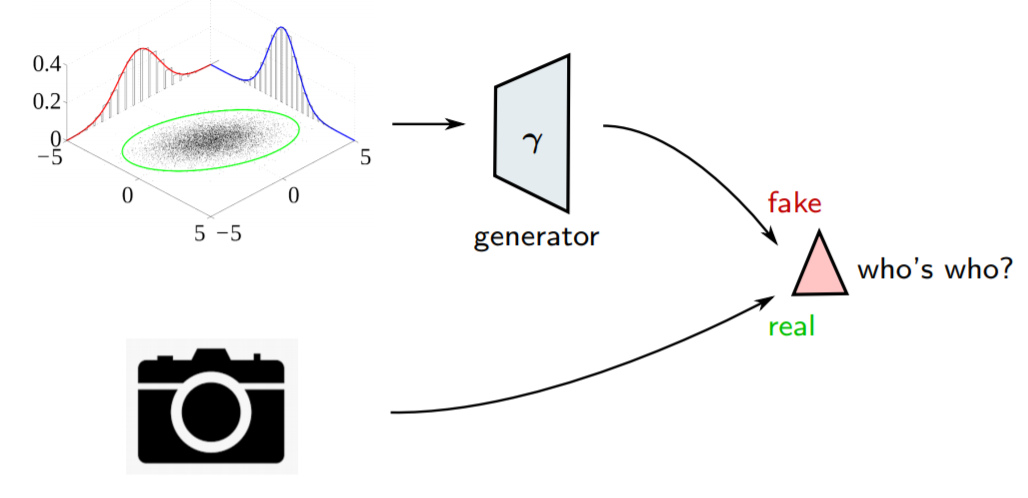
\includegraphics[width=.8\textwidth]{13/2_17}
	\caption{Decoder as a generator of fake samples.}\label{fig:13:1:gan}	
\end{figure}

Let's consider the situation depicted in \cref{fig:13:1:gan}. We have the decoder part of a VAE, parametrized by some parameters $\gamma$. This decoder acts as a \emph{generator}, since we can sample a random \emph{latent code} from the probability distribution defined over the latent space, supply it to the decoder that will decode it into a new (generated) sample in data space. How good is this generator at producing new samples? Our criterion is the \emph{realism} of the sample, i.e. how similar and indistinguishable it is from samples taken from real data, like real images. We will say that the sample produced by the generator is \emph{fake}, since it does not come from the real data distribution, while the real samples are, well, \emph{real}. Ideally, we would like our generator to be so good that no one could tell fake samples (generated by it) from the real samples apart.

Now, we would like to have a score that can be interpreted as the probability that a sample is real or not, to measure the goodness of the generator. However, how can we define such \emph{score}? Visual inspection is not enough of course. The key idea of \emph{Generative Adversarial Networks} (GAN) is that we can actually train a model, called \emph{discriminator}, to distinguish between real and fake samples.

\begin{figure}[H]
    \centering
    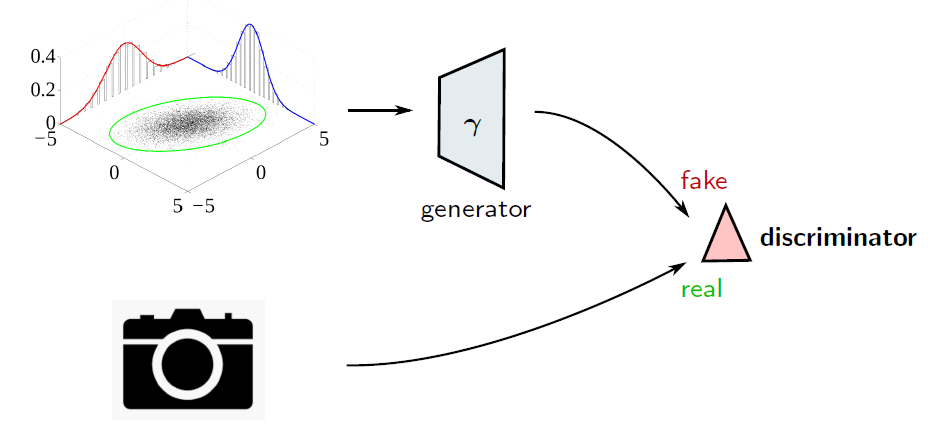
\includegraphics[width=.8\textwidth]{figures/13/gan-2.png}
    \caption{GAN.}
\end{figure}

We want to train a generator in such a way that a discriminator cannot distinguish between its generated sample and the real one. Simultaneously, we want to train a discriminator which is able to distinguish between fake samples and real ones. So, the generator and the discriminator are competing in a game: the generator tries to fool the discriminator and the discriminator tries to improve its proficiency in distinguishing forgeries from real data. They are \emph{adversaries}.

Both are implemented as deep neural networks, the generator parametrized by some parameters $\gamma$, and the discriminator by some parameters $\delta$. The task on which they are jointly trained, although with different objectives, is \emph{binary classification}. In fact, the discriminator will output a probability value for each sample, that will be used to classify the samples as one of two classes: \emph{real} or \emph{fake}.